\chapter{Single-atom resolved momentum measurement of lattice Bose gas}

blah blah blah

\section{Metastable Helium}

Metastable Helium, noted $\mathrm{He}^*$, is kind of an odd atom in the ensemble of species that we know how to bring to quantum degeneracy. Its most important feature, which is actually the reason why we chose this atom to measure correlation functions in momentum space, is the existence of the metastable state $2 \ ^3 S_1$. This excited state is called metastable for its very long lifetime of the order of $8,000 \ \mathrm{s}$, far larger than what is required for experiments. Very interestingly, as Helium is a noble gas, the amount of energy required to excite Helium into its metastable state is quite large, $19.8 \ \rm{eV}$. This large energy is sufficient for a metastable Helium atom to extract an electron from an electronic surface. This opens the way for \textbf{electronic detection} techniques, in opposition to the much more widely spread optical detection techniques, that allows for \textbf{single atom detection} as we will see in this chapter. In addition, the energy level structure (see Fig.-\ref{fig:niveaux}) is well adapted to laser cooling with a transition in the near-infrared around $\lambda_0 \simeq 1083 \ \mathrm{nm}$ for which reliable laser sources are available. Metastable Helium was actually amongst the first atoms to be brought to quantum degeneracy with the first BEC of $\He$ being obtained in 2001 simultaneously at the Institut d'Optique and Laboratoire Kastler Brossel in France. Helium also has the advantage to have a stable, albeit very rare and expensive fermionic isotope $^3 \He$ that has also been brought to quantum degeneracy at the Amsterdam LaserLab in 2006.

In spite of all these advantages, $\He$ comes with a few experimental difficulties that explain why they are actually quite few $\He$ experiments over the world. First, Helium is a very light atom and this comes with some very practical difficulties like the need for pre-cooling with liquid nitrogen and quite long Zeeman slowers. Second, $\He$ is subject to Penning collisions that bring back an atom to the ground state to ionize the other:

\begin{equation}
    \He + \He \rightarrow \mathrm{He} + \mathrm{He}^+ + \mathrm{e}^{-}
\end{equation}

Such a reaction thus results in the loss of two atoms and must be avoided. \NOTE{FINIR}

\begin{figure}
    \centering
    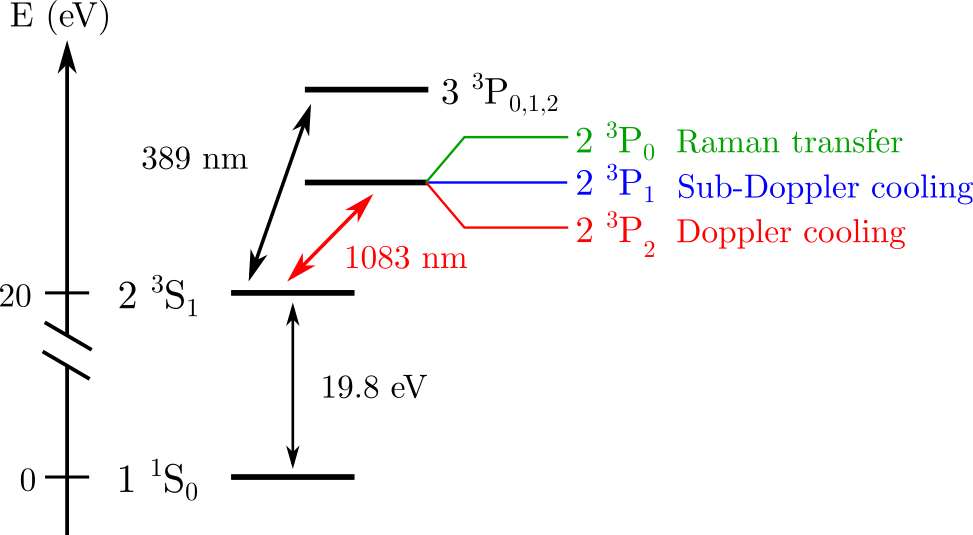
\includegraphics[width=0.9\textwidth]{Fig/Chapter3/niveaux.png}
    \caption{Energy levels of the Helium atom. The metastable state is the triplet state $2 \ ^3S_1$ that we will call the ground state of the metastable Helium atom. Laser cooling is performed on the optical transition $2 \ ^3S_1 \rightarrow 2 \ ^3 P$ of wavelength $\lambda_0 \simeq 1083 \ \mathrm{nm}$. More specifically, we address the transition to  $2 \ ^3 P_2$ or $2 \ ^3 P_1$ depending on the cooling scheme (respectively Doppler and sub-Doppler), as well as the transition to  $2 \ ^3 P_0$ to perform two-photon Raman transfer as we will detail later on.}
    \label{fig:niveaux}
\end{figure}

In the following, we will detail the different experimental steps used to bring a gas of metastable Helium to quantum degeneracy.

\section{Bose-Einstein Condensation of metastable helium}

\subsection{The source}

As the energy difference between the ground-state and the metastable state is very large, it is impossible to excite the atoms optically.

\begin{figure}
    \centering
    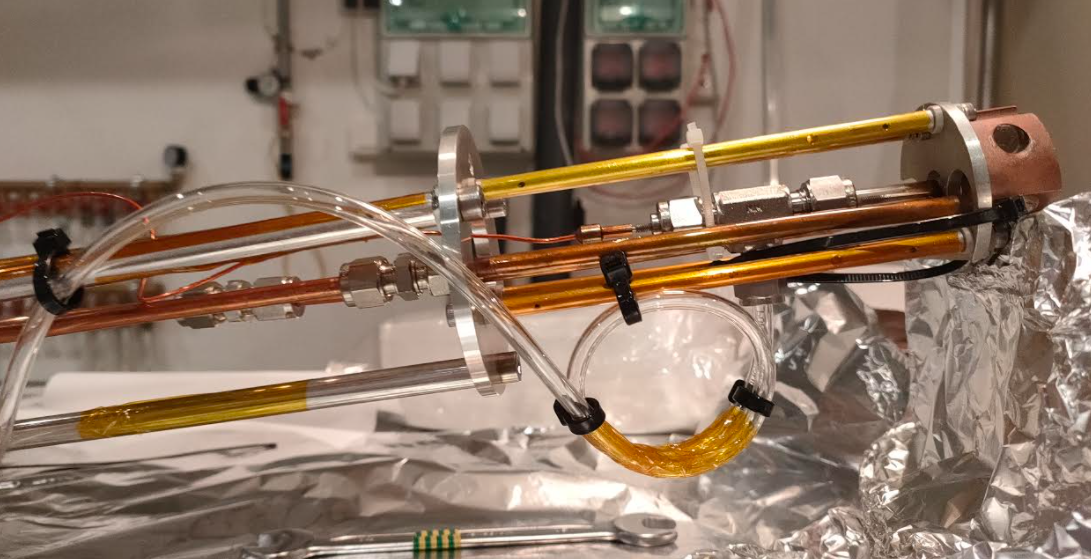
\includegraphics[width=0.9\textwidth]{Fig/Chapter3/source.png}
    \caption{Picture of the source apparatus.}
    \label{fig:my_label}
\end{figure}

\subsection{3D optical lattice}

\subsection{Electronic detection: The Micro Channel Plate Detector}

\section{Two-photon Raman transfer}

\subsection{Principle of the two-photon Raman transfer}

\subsection{Experimental implementation}

\section{Characterisation of two-body collisions in the time-of-flight dynamics}

\subsection{Classical model}

\subsection{Evolution with total atom number}

\subsection{Evolution with lattice depth}

\subsection{Conclusion}

\section{Adabiatic preparation in the vicinity of the Mott transition}

\subsection{Thermometry method}

\subsection{Fischer information and Cramér-Rao bound}

\subsection{Entropy measurement}
